\documentclass[11pt,a4paper,twoside]{article}
\usepackage[utf8]{inputenc}
\usepackage{polski}



\usepackage{graphicx}
\usepackage{subcaption} % obrazki obok siebie
%\usepackage[caption=false]{subfig} % obrazki nad sobą
\usepackage{wrapfig} 
\usepackage{float}
\usepackage{geometry}
%\geometry{lmargin=3cm,rmargin=2cm, tmargin=2.5cm, bmargin=2.5cm} %marginesy w pracy inż/mgr
\geometry{lmargin=2.5cm,rmargin=2.5cm, tmargin=2.5cm, bmargin=2.5cm} %marginesy ogólne
\usepackage{multirow} % scalanie wierszy tabeli

\usepackage{fancyhdr}
\pagestyle{fancy}
\fancyhead{} % wszystkie nagłówki puste
%\fancyhead[RE,LO]{ Absolwenci Wydziału Prawa  2012}
\fancyfoot{} % wszystkie stopki puste
\fancyfoot[LE,RO]{\thepage}
\renewcommand{\headrulewidth}{0pt}
%\renewcommand{\footrulewidth}{0.4pt}

\usepackage[hidelinks]{hyperref}% nazwy odsyłaczy

%unikanie myślników dzielących słowa między liniami
\tolerance=1
\emergencystretch=\maxdimen
\hyphenpenalty=10000
\hbadness=10000

\usepackage{algorithm}
\usepackage{algorithmicx}
\usepackage{algpseudocode}
\makeatletter
\renewcommand{\ALG@name}{Algorytm}
\renewcommand{\figurename}{Diagram}

\usepackage{enumitem}
\setitemize{itemsep=2pt,topsep=2pt,parsep=2pt,partopsep=2pt} %odstępy wyliczanych elementów (-)

\usepackage{indentfirst} % wcięcie w pierwszym akapicie (pod)rozdziału
%%%%%%%%%%%%%%%%%%%%%%%%%%%%%%%%%%%%%%%%% formatowanie kodu R
\usepackage{listings} 
\usepackage{color}
\definecolor{gray}{rgb}{0.5,0.5,0.5}
\lstset{
%language=Matlab,
basicstyle=\footnotesize\ttfamily,%\scriptsize\ttfamily,
columns=fullflexible,
keepspaces=true,
commentstyle=\ttfamily\color{gray},
numbers=left,
numberstyle=\ttfamily\color{gray}\footnotesize,
stepnumber=0, % numeracja linii
numbersep=5pt,
backgroundcolor=\color{white},
showspaces=false,
showstringspaces=false,
showtabs=false,
frame=none, % obramowanie kodu
tabsize=2,
captionpos=b,
breaklines=true,
breakatwhitespace=false,
title=\lstname,
escapeinside={},
keywordstyle={},
morekeywords={}
}
%%%%%%%%%%%%%%%%%%%%%%%%%%%%%%%%%%%%%%%%%

%%% zawijanie tekstu w tabelach zgodnie z życzeniem
\usepackage{stackengine}
\usepackage{array}
\newcolumntype{L}[1]{>{\raggedright\arraybackslash}p{#1}}
\setstackEOL{\#}
\setstackgap{L}{12pt}
%%%

\usepackage{amsfonts} % zbiory liczba (np. naturalnych)
\usepackage{amsmath} %duże klamry
\usepackage{bbm} %skok jednostkowy
\usepackage[titletoc,title]{appendix} % dodatki - zmiana wyświetlania nagłówka
\pagenumbering{gobble}
\usepackage{afterpage} % pusta strona
\usepackage{tabularx}

\usepackage{makecell}

%\usepackage{setspace} % interlinia
%\singlespacing 
%\onehalfspacing
%\doublespacing
%\setstretch{0.96}

\begin{document}


\begin{center}
\vspace*{3\baselineskip}
{\LARGE{RSO Projekt}}
\\
\vspace*{2\baselineskip}
{\Large{Sklep internetowy}}
\\
\vspace*{2\baselineskip}
\begin{table}[ht]
%\caption{Rejestr zmian}
\label{autors}
\centering
\begin{tabular}{ll}
	Szymon Bezpalko & 269265\\
	Konrad Kaproń & 269304\\
	Tomasz Korzeniowski & 265753\\
	Marcin Macias & 269328\\
	Krzysztof Solecki & 269346\\
	Michał Trochimiak & 265780\\
\end{tabular}
\end{table}

%Szymon Bezpalko, 269265\\
%Konrad Kaproń, 269304\\
%Tomasz Korzeniowski, 265753\\
%Marcin Macias, 269328\\
%Krzysztof Solecki, 269346\\
%Michał Trochimiak, 265780\\
\vspace*{2\baselineskip}
\today
\end{center}
\vspace*{3\baselineskip}
\begin{center}
Rejestr zmian
\end{center}

%\bgroup
%\def\arraystretch{1.1}
\begin{table}[ht]
%\caption{Rejestr zmian}
\label{changelog}
\centering
\begin{tabular}{|c|c|l|}
\hline
 Data & Wersja & \multicolumn{1}{c|}{Zmiany} \\\hline
 29.03.2018 & 0.1 & Utworzenie dokumentacji, specyfikacja i analiza wymagań \\\hline
 19.04.2018 & 0.2 & Opracowanie wstępnych interfejsów serwisów i wyglądu aplikacji użytkowej \\\hline
 26.04.2018 & 0.3 & Szczegółowy opis serwisów \\\hline
 10.05.2018 & 1.0 & Dokumentacja etapu pierwszego\\\hline
\end{tabular}
\end{table}
%\egroup
\newpage
\tableofcontents

%\afterpage{\null\newpage}

\clearpage
\pagenumbering{arabic}
\setcounter{page}{3}

\section{Specyfikacja wymagań}
Tworzony system informatyczny powinien realizować podstawowe funkcjonalności sklepu internetowego. Jego głównym zadaniem jest umożliwienie katalogowania produktów oferowanych przez dostawcę (producenta) oraz przechowywanie informacji o zamówieniach realizowanych przez klientów. 

Przez katalogowanie produktów należy rozumieć przechowywanie informacji na temat produktów oferowanych przez danego dostawcę wraz z możliwością dodawania nowych i modyfikowania już istniejących produktów. Klienci systemu powinni mieć możliwość wyszukiwania interesujących ich produktów na podstawie wybranych kryteriów (jak cena czy rodzaj towaru) oraz dodawania ich do koszyka. Koszyk jest definiowany jako zbiór produktów, które klient wybrał w celu ich zakupu, lecz jeszcze nie zatwierdził ich w celu płatności. Przed dokonaniem zamówienia, klient może zrezygnować z części lub wszystkich elementów koszyka. Po zatwierdzeniu wszystkich elementów koszyka, klient dokonuje zamówienia. Złożone zamówienie może być wyświetlane przez zamawiającego, a także modyfikowane przez określony czas.

Do zadań systemu należy zaliczyć także możliwość generowania podstawowych statystyk dotyczących sprzedaży wybranych produktów. Jest to jednak wymaganie opcjonalne, gdyż głównym celem tworzonego systemu jest dostarczenie funkcjonalności odpowiadających za  zakup towarów. Za realizację płatności za zamówienie odpowiedzialny będzie system zewnętrzny.

W systemie przechowywane są dane osobowe klientów i dostawców. Muszą one być przechowywane w sposób bezpieczny, zabezpieczony przed dostępem osób niepowołanych, a także zgodnie z wymogami ustawy o ochronie danych osobowych. W szczególności, każdemu podmiotowi, którego dane figurują w systemie, przysługuje prawo do żądania ich modyfikacji lub usunięcia. Usuwanie dotyczy jednak tylko danych osobowych, a nie wszystkich powiązanych z danym podmiotem informacji zapisanych w systemie.

Projektowany system, w swojej podstawowej wersji, powinien być nastawiony na obsługę producentów napojów alkoholowych. Projekt powinien być jednak na tyle uniwersalny by można było łatwo wykorzystać wytworzone rozwiązanie do sprzedaży innych rodzajów towarów (wraz z rozwojem firmy/systemu lub udostępnienia rozwiązania innym usługodawcom).

\section{Analiza wymagań}
\subsection{Wymagania funkcjonalne}
\begin{enumerate}[start=1,label={WF\arabic*.}]
\item W związku z koniecznością umożliwienia dostępu do systemu dostawcom produktów oraz klientom, konieczne jest stworzenie mechanizmu kont użytkowników, wraz z możliwością ich edytowania i kasowania. Za utworzenie konta w systemie odpowiedzialny jest użytkownik systemu. Wyróżnia się dodatkowe konto administratora, które umożliwi rozwiązywanie problemów dotyczących użytkowania systemu (w tym zakładania kont, ich nadzorowanie i edycja) a także nadzorowania poprawności działania systemu.
\item Administrator systemu ma możliwość dodania, usunięcia i zmiany danych osobowych użytkownika. Przyjmuje się, że usunięcie danych osobowych następuje tylko w sytuacji, gdy osoba, której dane dotyczą, wystąpi z żądaniem o zaprzestanie ich przetwarzania. W przeciwnym razie (np. zaprzestanie korzystania z systemu wraz z unieważnieniem konta (np. producent zbankrutował, więc już nie będzie dostarczał produktów)) dane nie są usuwane, a jedynie zostaje zmieniony ich status. Dzięki temu możliwa jest archiwizacja danych dotyczących zawartych transakcji.
\item Dostawcy produktów mają możliwość dodawania i modyfikowania informacji dotyczących oferowanych towarów. W ramach dodawania produktów istnieje możliwość dodawania pojedynczego produktu, a także wielu produktów zebranych w ustrukturyzowanym pliku. Modyfikowanie produktu uwzględnia  zmianę jego opisu, a także informacje o jego cenie i dostępności. Usuwanie produktu polega na zaprzestaniu wyświetlania produktu w interfejsach użytkowników oraz zmianie statusu produktu zamiast jego trwałego usunięcia. Powyższe funkcjonalności dostępne są także dla administratora systemu.
\item Zalogowany użytkownik ma możliwość tworzenia koszyka produktów. W tym celu korzysta z możliwości wyszukiwania produktów na podstawie wybranych kryteriów (cena, rodzaj towaru, dostępność), przeglądania szczegółowych informacji o wybranym produkcie, a także dodawania go do koszyka. Produkty znajdujące się w koszyku mogą być modyfikowane co do zamawianej ilości oraz usuwane z koszyka. Zatwierdzenie składu koszyka jest jednoznaczne ze złożeniem zamówienia.
\item Złożone zamówienie może być przeglądane i modyfikowane przez klienta. Modyfikacja udostępniana jest tylko przez pewien czas, zależny od momentu złożenia zamówienia (realizacja zamówień odbywa się o ustalonych godzinach, pod warunkiem dokonania opłaty za zamówienie). Modyfikacji podlega ilość zamówionego produktu. Klient ma również możliwość anulowania zamówienia, o ile nie rozpoczęła się jego realizacja. (zakładamy, że dla reklamacji i zwrotów produktów powstanie nowy mikroserwis). 
\item System powinien mieć możliwość generowania raportów i statystyk dotyczących sprzedaży produktów. Funkcjonalność ta dostępna jest dla dostawców produktów.
\end{enumerate}

\subsection{Wymagania niefunkcjonalne}
\subsubsection{Użyteczność}
\begin{enumerate}[start=1,label={WNF\arabic*.}]
\item Wszystkie elementy systemu powinny udostępniać użytkownikom jednolity interfejs graficzny. Z systemu można korzystać zarówno w języku polskim, jaki i angielskim.
\end{enumerate}
\subsubsection{Niezawodność i bezpieczeństwo}
\begin{enumerate}[start=2,label={WNF\arabic*.}]
\item Dane osobowe wszystkich podmiotów, które są przechowywane w systemie, muszą być składowane zgodnie z wymogami ustawy o ochronie danych osobowych. 
\item Hasła do kont użytkowników przechowuje się w sposób bezpieczny, uniemożliwiający wykradzenie, używając funkcji skrótu zgodnie ze standardem SHA3.
\item Całość systemu powinna działać możliwie niezawodnie i cechować się odpornością na awarie. Stosowana będzie redundancja danych w celu umożliwienia odtworzenia wszystkich informacji przechowywanych w systemie po ewentualnej awarii. Czas przywracania funkcjonalności systemu w przypadku awarii lub ataku nie powinien być dłuższy niż 24 godziny, a czas pomiędzy wystąpieniami awarii nie powinien być krótszy niż 6 miesięcy.
\item System powinien przesyłać przez sieć jakiekolwiek dane dotyczące podmiotów oraz informacje dostępowe w stanie zaszyfrowanym.
\item System powinien być odporny na znane ataki, w tym:  injection, brute force, forced browsing, XSS, XST
\item Wszystkie wysłane do systemu pliki powinny być najpierw automatycznie sprawdzane w systemie typu sandbox.
\item System powinien stosować zasadę najmniejszych uprawnień.
\item W czasie użytkowania systemu stosowane zabezpieczenia powinny być uaktualniane.
\item System powinien mieć możliwość tworzenia kopii zapasowych nie rzadziej niż codziennie w godzinach nocnych.
\end{enumerate}
\subsubsection{Wydajność}
\begin{enumerate}[start=11,label={WNF\arabic*.}]
\item System musi umożliwiać wydajną jednoczesną pracę 5000 klientów oraz 200 dostawców produktów. Czas odpowiedzi systemu przy takim obciążeniu nie może przekraczać pięciu sekund, tj. czasu od otrzymania żądania przez serwer do wysłania odpowiedzi.
\item System powinien być przygotowany do łatwej rozbudowy zarówno w sferze sprzętowej, jak i programowej. Powinien być także skalowalny, tj. zostać zaprojektowany w taki sposób, by w przyszłości liczba użytkowników mogła wzrosnąć bez konieczności jego znaczącej przebudowy.
\end{enumerate}

\section{Przypadki użycia}
Na podstawie specyfikacji oraz wymagań funkcjonalnych wyodrębnionych w czasie analizy, można wyróżnić następujących aktorów systemu:
\begin{itemize}[label={--}]
\item Klient - osoba fizyczna lub firma dokonująca zamówień w systemie (zalogowany)
\item Dostawca produktu - osoba fizyczna lub firma oferująca produkty (zalogowany)
\item Anonimowy użytkownik - odwiedzający stronę systemu (niezalogowany)
\item Administrator systemu
\item Inne systemy - system płatności za zamówienia, system reklamacji i zwrotów produktów
\end{itemize}

\vspace*{1\baselineskip}
Zdefiniowano następujące przypadki użycia systemu:
\begin{enumerate}[start=1,label={PU\arabic*.}]
\item \textbf{Rejestracja użytkownika:} Stworzenie konta użytkownika, obejmuje nadanie mu nazwy i hasła oraz odpowiednich uprawnień.
\item \textbf{Modyfikacja konta użytkownika:} Użytkownik może zmienić hasło lub dane osobowe.
\item \textbf{Wyrejestrowanie użytkownika:} Zmiana stanu konta użytkownika.
\item \textbf{Usunięcie danych użytkownika:} Trwałe usunięcie danych osobowych użytkownika, wykonywane jedynie na jego żądanie zaprzestania przetwarzania danych osobowych. Nie oznacza to usunięcia konta ani innych informacji związanych z jego użytkowaniem.
\item \textbf{Logowanie do systemu:} Dowolny użytkownik może zalogować się do systemu poprzez podanie nazwy użytkownika i aktualnego hasła.
\item \textbf{Wylogowanie z systemu:} Zalogowany użytkownik może zakończyć pracę z systemem, tracąc możliwość dostępu do przechowywanych w nim danych, poprzez wybór opcji wylogowania.
\item \textbf{Dodanie produktu:} Dostawca produktu definiuje nowy produkt (lub listę produktów), który będzie oferował. 
\item \textbf{Modyfikacja produktu:} Dostawca produktu może zmienić informacje szczegółowe o produkcie, w tym dostępną ilość produktu i jego cenę
\item \textbf{Usuwanie produktu:} Dostawca produktu usuwa dotychczasowy produkt. Nie jest on widoczny w interfejsie użytkownika, lecz informacje o nim pozostają zapisane w systemie.
\item \textbf{Wyszukiwanie produktu:} Dowolny użytkownik systemu może przeglądać katalog produktów, a po wybraniu interesującego produktu może przeglądać jego szczegółowe informacje.
\item \textbf{Dodawanie produktu do koszyka:} Klient wyszukuje produkt, który zamierza dodać do koszyka produktów. 
\item \textbf{Modyfikacja koszyka produktów:} Klient może zmieniać ilość zamawianych produktów a także usuwać wskazane pozycje.
\item \textbf{Złożenie zamówienia:} Klient dokonuje weryfikacji swojego koszyka produktów i zatwierdza jego zawartość.
\item \textbf{Modyfikacja zamówienia:} Klient dokonuje zmiany ilości zamawianego produktu, o ile realizacja zamówienia nie została rozpoczęta.
\item \textbf{Anulowanie zamówienia:} Klient rezygnuje ze złożonego zamówienia, o ile jego realizacja nie została rozpoczęta.
\item \textbf{Wyszukiwanie zamówienia:} Klient i dostawca produktu mogą przeglądać dotychczas złożone zamówienia.
\item \textbf{Generowanie statystyk i raportów:} Dostawca produktu może wygenerować statystyki i raporty opisujące zamówienia wskazanych produktów
\end{enumerate}

\section{Architektura systemu}
%Ogólnie o architekturze mikroserwisów, wzorce architektoniczne z jakich korzystamy, decyzje architektoniczne, które wpływają na system
%\\
%\\
\begin{figure}[ht]
%\vspace{-20pt}
\caption{Diagram klas}
\label{diagramKlas}
\centering
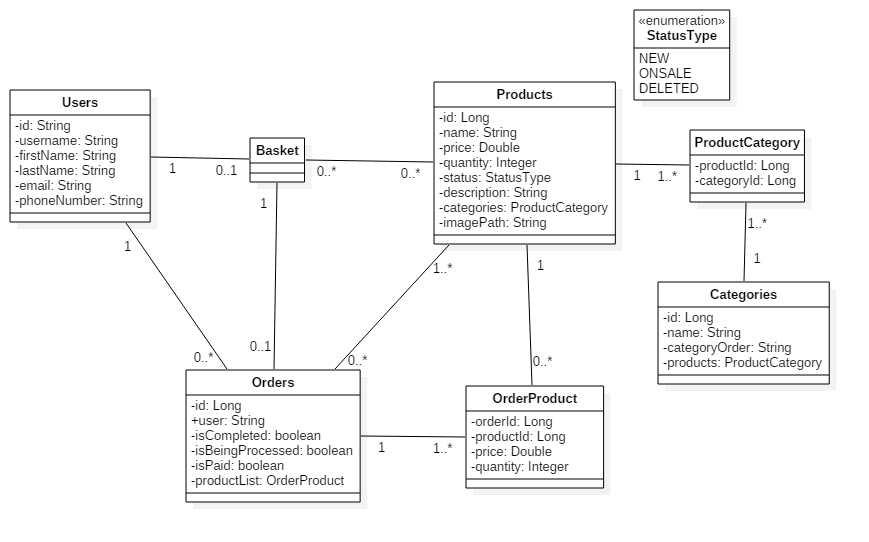
\includegraphics[height=8.4cm, width=15.7cm]{Klasy}
\end{figure}

%\begin{figure}[ht]
%%\vspace{-20pt}
%\caption{Diagram pakietów}
%\label{diagramPakietow}
%\centering
%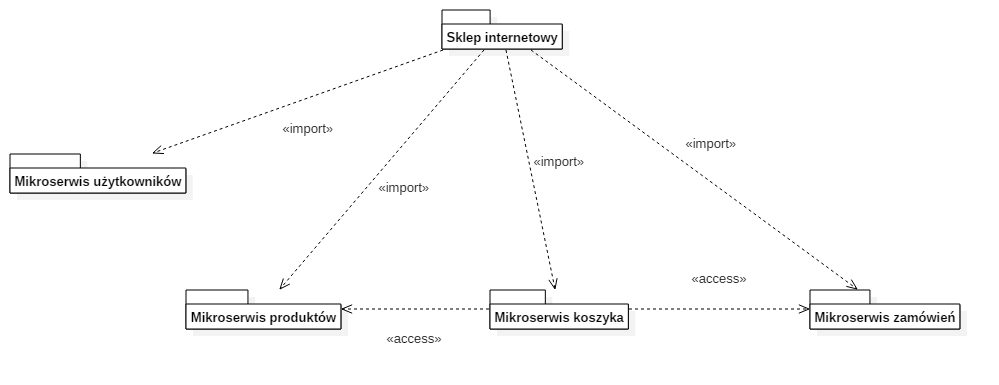
\includegraphics[height=7.4cm, width=15.7cm]{Pakiety}
%\end{figure}

\begin{figure}[ht]
%\vspace{-20pt}
\caption{Główny proces biznesowy}
\label{procesBiznesowy01}
\centering
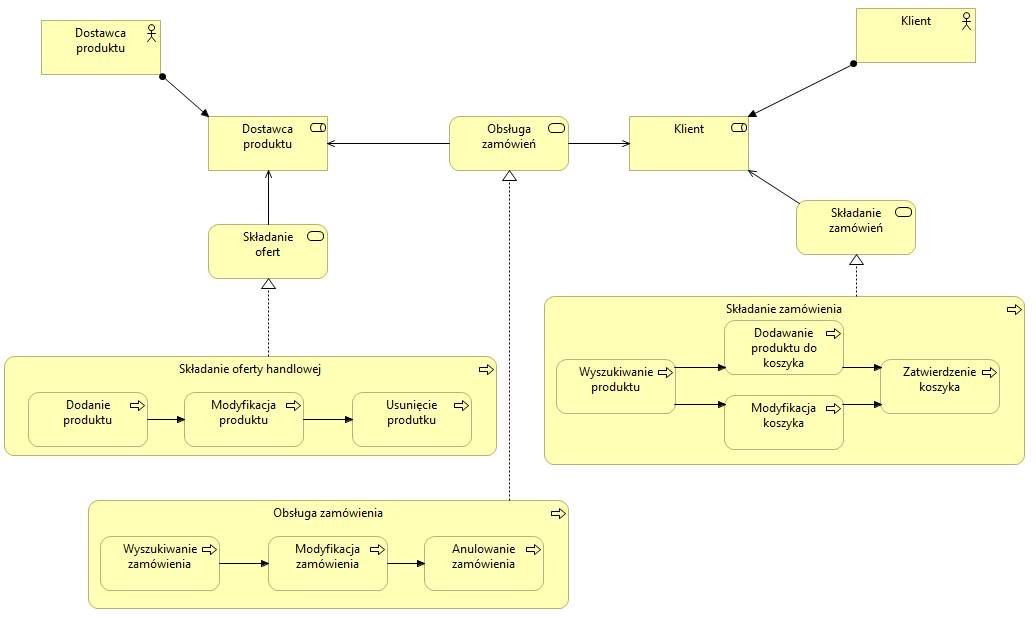
\includegraphics[height=12cm, width=15.7cm]{01_biznes}
\end{figure}

\begin{figure}[ht]
%\vspace{-20pt}
\caption{Realizacja dodawania i modyfikacji produktów przez dostawców}
\label{dodawanieProduktu02}
\centering
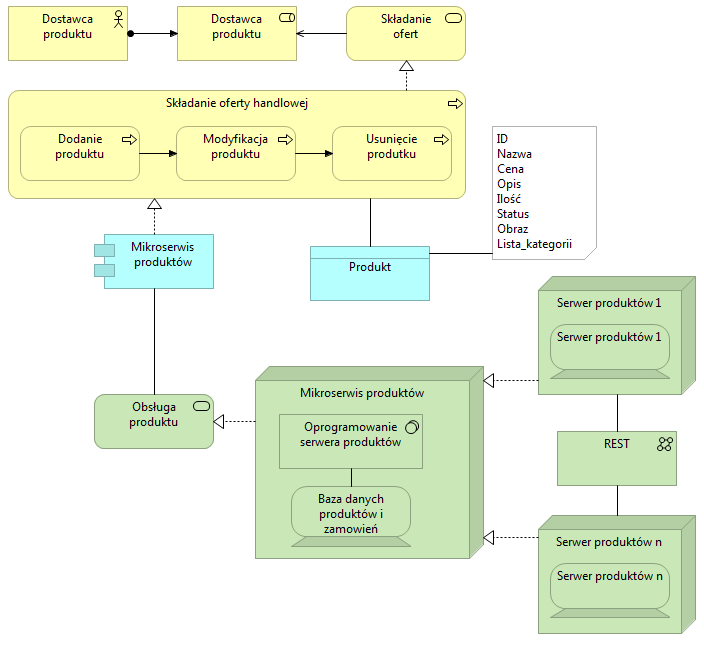
\includegraphics[height=10.3cm, width=15.7cm]{02_produkt}
\end{figure}

\begin{figure}[ht]
%\vspace{-20pt}
\caption{Składanie zamówień przez klientów}
\label{skladanieZamowienia03}
\centering
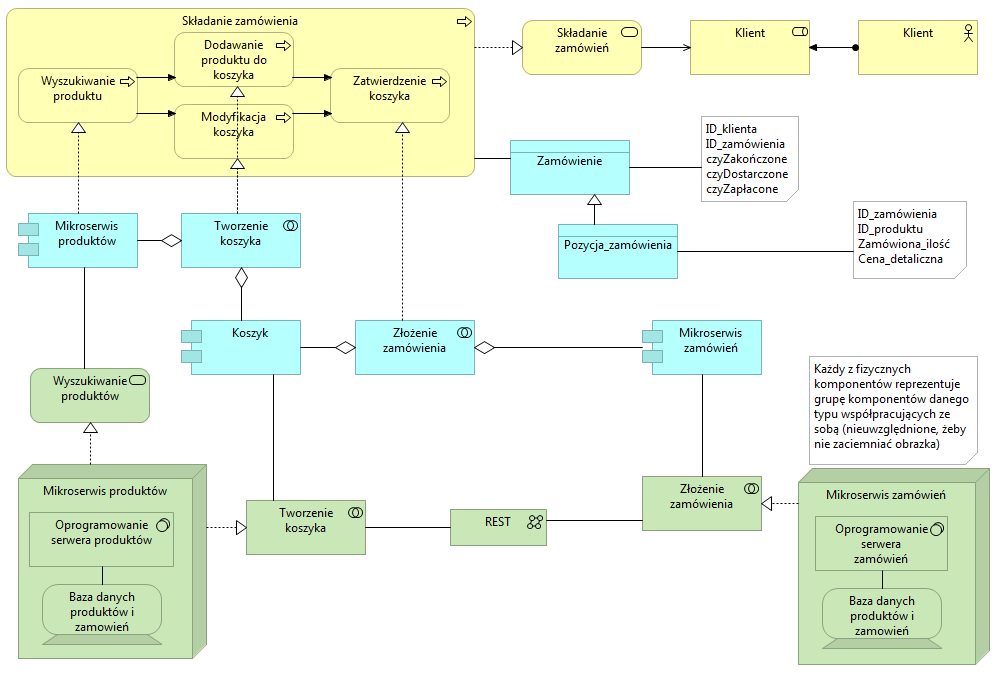
\includegraphics[height=11.5cm, width=15.7cm]{03_zamowienie_skladanie}
\end{figure}

\begin{figure}[ht]
%\vspace{-20pt}
\caption{Obsługa już istniejących zamówień}
\label{obslugaZamowienia04}
\centering
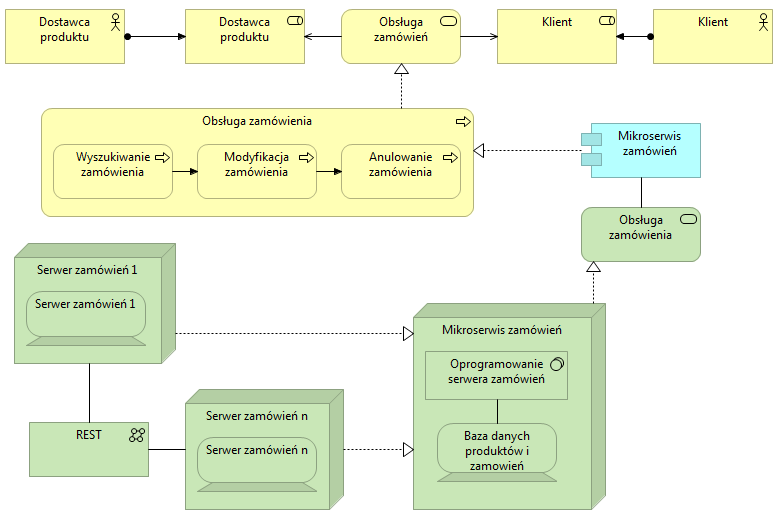
\includegraphics[height=11cm, width=15.7cm]{04_zamowienie_obsluga}
\end{figure}

\clearpage
\section{Rozwiązanie}
W ramach projektów powstały następujące serwisy:

\begin{table}[ht]
%\caption{Rejestr zmian}
\label{spisSerwisow}
\centering
\begin{tabular}{|l|l|l|}
\hline
 Nazwa & Webservice & Panel wildfly \\\hline
 Frontend & localhost:80 & -- \\\hline
 Keycloak & localhost:8080/auth/admin & -- \\\hline
 User-webservice & localhost:8081/user-webservice-rest/api & localhost:9991 \\\hline
 Product-webservice & localhost:8082/product-webservice-rest/api & localhost:9992 \\\hline
 Order-webservice & localhost:8082/order-webservice-rest/api & localhost:9993\\\hline
 Testowy wildfly & localhost:8089/* & localhost:9999 \\\hline
\end{tabular}
\end{table}

\subsection{Serwis użytkowników}
Serwis udostępnia dane użytkowników, pozwala też na ich dodawanie, edycję oraz usuwanie. Do działania konieczne jest uruchomienie Keycloak'a  - serwis nie komunikuje się bezpośrednio z bazą danych w której zapisane są dane użytkowników, zamiast tego służy jako proxy pomiędzy Keycloak'iem a pozostałymi modułami.

Użytkownicy opisani są następującą strukturą:

\begin{lstlisting}
User
{
  "id": "1333edbb-c0c6-42ae-8852-c9c10f5c6f8d",
  "username": "jkowalski",
  "firstName": "Jan",
  "lastName": "Kowalski",
  "email": "jkowalski@gmail.com",
  "phoneNumber": "123456789",
  "roles": ["user"]
}
\end{lstlisting}
\vspace{-20pt}
Obecnie przewidziane są dwie role użytkowników - user oraz admin. ID użytkowników jest reprezentowany przez GUID zgodny ze standardem RFC 4122. Jego wartość jest przekazywana wraz z tokenem dostępu. Jeśli zajdzie konieczność powiązania jakichś danych z użytkownikami w bazach innych serwisów, zapisany zostanie GUID, natomiast dane personalne (w tym nazwa użytkownika) będzie można uzyskać tylko przy komunikacji z serwisem użytkowników.

Nazwa użytkownika oraz email są unikalne, wartości pozostałych atrybutów mogą się powtarzać. ID oraz nazwa użytkownika nie mogą być zmieniane. Zarówno id, jak i nazwa roli są unikalne.

Diagram \ref{userDB} przedstawia tabele których dane udostępnia serwis użytkowników.

\begin{figure}[ht]
%\vspace{-20pt}
\caption{Schemat bazy danych serwisu użytkowników.}
\label{userDB}
\centering
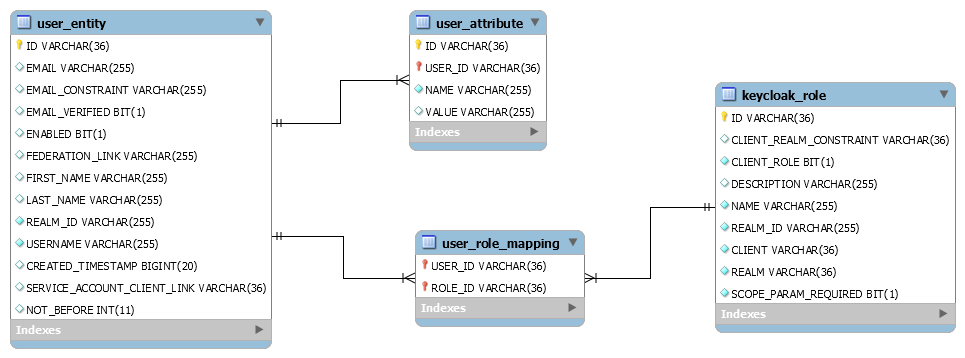
\includegraphics[height=5.5cm, width=15.7cm]{userDB}
\end{figure}

Funkcje udostępniane przez serwis użytkowników zawiera tabela \ref{funkcjeUserWebservice}.
\begin{table}[htp]
\caption{Funkcje udostępniane przez serwis użytkowników}
\label{funkcjeUserWebservice}
\centering
%\begin{tabular}{|l|l|l|l|l|l|l|}
\begin{tabularx}{\textwidth}{|X|c|c|X|X|l|c|}
\hline
 Funkcja & \makecell{Wymagana \\ rola} & Metoda & Adres & Parametry zapytania & Body \\\hline
 Pobierz dane użytkownika & user & GET & /api/users/{userId} & -- & -- \\\hline
 Pobierz dane użytkowników & admin & GET & /api/users & \ref{stdZapytan} (tylko eq/ne/in/lk) & -- \\\hline
  Dodaj użytkownika & user & POST & /api/users & -- & User \\\hline
   Zmień dane użytkownika & user & PUT & /api/users & -- & User \\\hline
    Przydziel rolę użytkownikowi & admin & PUT & /api/users/{userId} /roles/add & String roleName & -- \\\hline
     Odbierz rolę użytkownikowi & admin & PUT & /api/users/{userId} /roles/remove & String roleName & -- \\\hline
      Usuń użytkownika & user & DELETE & /api/users & -- & User \\\hline
  Ustaw hasło użytkownika & user & PUT & /api/users/{userId} /resetPassword & \makecell{String userId,\\ newPassword} & -- \\\hline
\end{tabularx}
\end{table}

Uwagi dotyczące korzystania z serwisu:
\begin{enumerate}
\item W przypadku funkcji w których wymagana jest jedynie rola user, dodatkowo w serwisie sprawdzane będzie czy id użytkownika w tokenie podanym przy zapytaniu odpowiada id użytkownika, który ma być odczytany, zmieniony czy usunięty.
\item W przypadku dodawania użytkownika ignorowane jest pole id oraz roles (id zostanie wygenerowane automatycznie i zwrócone w odpowiedzi).
\item W przypadku edycji lub usuwania użytkownik identyfikowany jest przez pole id. Przy edycji pola username oraz roles są ignorowane.
\item Każdy użytkownik w systemie domyślnie posiada rolę user (od razu po dodaniu).
\item Po dodaniu nowego użytkownika konieczne jest skorzystanie z funkcji ustawiającego jego hasło, korzystając z id zwróconego w odpowiedzi (w innym przypadku nie jest możliwe logowanie).
\end{enumerate}

\subsection{Serwis produktów}
Serwis udostępniający dane o produktach i umożliwiający ich dodawanie oraz edycję. Produkt oferowany przez serwis opisany jest następującą strukturą:

\begin{lstlisting}
Product:
{
 "id": 41,
 "name": "Platonowek",
 "price": 9.99,
 "quantity": 100,
 "status": "new",
 "description": "Najlepsze piwerko",
 "categories": [
                {
                    "productId": 41,
                    "categoryId": 1
                },
                {
                    "productId": 41,
                    "categoryId": 3
                }
            ]
 "imagePath":"sciezka/do/pliku.jpg"
}
\end{lstlisting}
\vspace{-20pt}
Identyfikator produktu jest niezmienną liczbą naturalną generowaną automatycznie podczas dodawania produktu do bazy danych. Nazwa, opis produktu oraz cena są ważne z punktu widzenia wyświetlania tych danych klientowi. Dostępna ilość wskazuje ile produktów oferowanych jest przez wszystkich dostawców sklepu (wartość ustalana przez serwis zamówień/dostaw). Ścieżka pod którą znajduje się obraz oraz statusy produktu są parametrami technicznymi. Możliwe statusy opisuje poniższa struktura danych:

\begin{lstlisting}
public static enum StatusType { NEW, ONSALE, DELETED }
\end{lstlisting}
\vspace{-20pt}
Znaczenie statusów produktów:
\begin{enumerate}
\item NEW -- produkt w bazie danych, lecz jeszcze nie w sprzedaży
\item ONSALE -- produkt w sprzedaży
\item DELETED -- produkt usunięty (produkty nigdy nie są fizycznie usuwane z bazy)
\end{enumerate}

Każdy produkt może należeć do wielu kategorii, a kategorie naturalnie zawierają wiele produktów. Kategorie produktów zawiera tabela ProductCategory

\begin{lstlisting}
ProductCategory: {"productId": 41, "categoryId": 1}
\end{lstlisting}
\vspace{-20pt}

Kategorie produktów przechowywane są w tabeli Categories:

\begin{lstlisting}
Category:
{
"id": 7,
"name": "kolejne-poziomy-oddzielane-myslnikami",
"categoryOrder": "2.0",
"products": [
		{
			"productId": 1,
            "categoryId": 7
		},
        {
			"productId": 2,
			"categoryId": 7
        },
        {
			"productId": 5,
			"categoryId": 7
        },
            ]
}
\end{lstlisting}
\vspace{-20pt}

Można na jej podstawie znaleźć wszystkie produkty należące do wybranej kategorii. categoryOrder odpowiada za poziomy listy grupującej kategorie produktów na ekranie

Klasy Product oraz Order odpowiadają schematowi bazy danych (diagram \ref{productDB}), z którego korzysta serwis.

\begin{figure}[ht]
%\vspace{-20pt}
\caption{Schemat bazy danych serwisu użytkowników.}
\label{productDB}
\centering
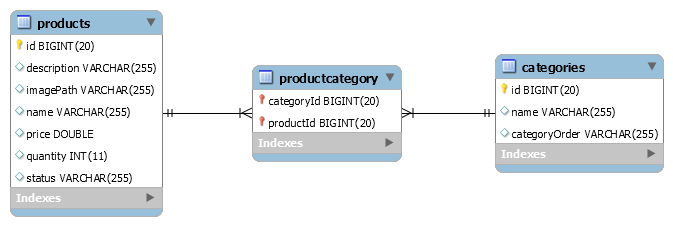
\includegraphics[height=4.5cm, width=15.7cm]{productDB}
\end{figure}

Funkcje udostępniane przez serwis produktów zawiera tabela \ref{funkcjeProductWebservice}.
\begin{table}[htp]
\caption{Funkcje udostępniane przez serwis produktów}
\label{funkcjeProductWebservice}
\centering
%\begin{tabular}{|l|l|l|l|l|l|l|}
\begin{tabularx}{\textwidth}{|X|c|X|X|c|c|}
\hline
 Funkcja & Metoda & Adres & \makecell{Parametry \\ zapytania} & Body \\\hline
 Wyszukaj produkty & GET & /api/products & \ref{stdZapytan} & -- \\\hline
 Dodaj produkt & POST & /api/products /add & -- & Product \\\hline
 Dodaj listę produktów & POST & /api/products /addList & -- & List$<$Product$>$ \\\hline
 Zmień wartości atrybutów & PUT & /api/products /update & -- & Product \\\hline
 Dodaj kategorię produktu & PUT & /api/products /updateCategory & \makecell{Long productId, \\ Long categoryId} & -- \\\hline
 Usuń kategorię produktu & DELETE & /api/products /deleteCategory & \makecell{Long productId, \\ Long categoryId} & -- \\\hline
 Usuń listę kategorii produktu & DELETE & /api/products/ deleteCategoryList & -- & \makecell{List \\ $<$ProductCategory$>$} \\\hline
 Usuń produkt & PUT & /api/products /delete & \makecell{Long productId} & -- \\\hline
 Usuń listę produktów & PUT & /api/products /deleteList & -- & List$<$Long$>$ \\\hline
 Wyszukaj kategorie (wraz z listą produktów) & GET & /api/products /getCategory & \ref{stdZapytan} & -- \\\hline
 Wyszukaj wszystkie kategorie (bez listy produktów) & GET & /api/products/ getCategoryNames & -- & -- \\\hline
 Zarezerwuj produkty do zamówienia & PUT & /api/products /makeOrder & -- & \makecell{List \\ $<$OrderPosition$>$} \\\hline
 Anuluj zamówione produkty & PUT & /api/products /deleteOrder & -- & \makecell{List \\ $<$OrderPosition$>$} \\\hline
\end{tabularx}
\end{table}

Rezerwowanie produktów (podczas obsługi zamówienia) obejmuje sprawdzenie czy każda pozycja zamówienia na liście spełnia poniższe warunki:
\begin{enumerate}
\item identyfikator produktu musi znajdować się w bazie produktów. Jeśli identyfikator nie istnieje w bazie, jest on zwracany do serwisu zamówień.
\item cena produktu w zamówieniu musi być zgodna z ceną produktu w bazie. Jeśli klient, podczas składania zamówienia, zaakceptował inną cenę niż produkt faktycznie posiada, serwis zamówień otrzymuje identyfikator produktu wraz z aktualną ceną oferowaną w sklepie
\item ilość zamawianego produktu nie może być większa od dostępnej ilości produktu w sklepie. Jeśli klient zażąda zbyt dużej ilości produktu, serwis zamówień zostanie powiadomiony o identyfikatorze takiego produktu oraz aktualnej dostępnej ilości produktu w sklepie.
\end{enumerate}

Możliwe są wszystkie dopuszczalne kombinacje niespełnienia powyższych warunków, a każda pozycja je naruszająca zostaje zwrócona do serwisu zamówień. W każdym z takich przypadków całe zamówienie nie zostanie potwierdzone jako zaakceptowane przez bazę produktów.

\begin{lstlisting}
OrderPosition:
{
	"productId": 7,
    "price": null,
    "quantity": 19
}
\end{lstlisting}
\vspace{-20pt}
\subsection{Serwis zamówień}
Serwis realizujący obsługę zamówień; ich składanie, edycję, dostęp oraz anulowanie. Zamówienia opisane są następującą strukturą:

\begin{lstlisting}
Order:
{
	"id": 2137,
    "userId": 12,
    "isCompleted": true,
    "isBeingProcessed": false,
    "isPaid" : true,
    "productsList": 
    [
    	{
        	"orderId": 2137,
        	"productId": 1,
            "price": 2.49,
            "quantity": 30
        },
        {
        	"orderId": 2137
            "productId": 2,
            "price": 2.49,
            "quantity": 20
        }
    ]
}
\end{lstlisting}
\vspace{-20pt}
"id" jest liczbą całkowitą generowaną automatycznie pełniąca rolę klucza głównego w serwisie zamówień, "userId" jest napisem oznaczającym identyfikator użytkownika. Będzie on otrzymywany z serwisu użytkowników. Kolejne trzy zmienne reprezentują stan zamówienia. Zamówienie może znajdować się w stanach opisanych w tabeli \ref{stanyZamowienia}.

\begin{table}[htp]
\caption{Stany zamówienia.}
\label{stanyZamowienia}
\centering
\begin{tabularx}{\textwidth}{|c|c|c|X|}
\hline
 Zakończone & Opłacone & \makecell{W trakcie \\ przesyłki} & Stan zamówienia \\\hline
 1 & 1 & 0 & Dostarczone do klienta. \\\hline
 0 & 1 & 1 & W trakcie dostarczania do klienta, niemożliwe anulowanie transakcji. \\\hline
 0 & 0 & 1 & W trakcie dostarczania do klienta. Niemożliwe anulowanie transakcji (płatność gotówką). \\\hline
 0 & 1 & 0 & Zamówienie nie jest w trakcie dostarczania do klienta. Możliwe anulowanie transakcji oraz zwrot wpłaconej kwoty. \\\hline
 0 & 0 & 0 & Zamówienie nie jest w trakcie dostarczania do klienta. Możliwe anulowanie transakcji. \\\hline
\end{tabularx}
\end{table}

Zamówienie zawiera listę produktów. Każdy z produktów zawiera pole "productId", reprezentujące jego identyfikator, pole "quantity" określające ilość zamawianego produktu, oraz pole "price" specyfikujące koszt jednostkowy danego towaru. Wystąpienia poszczególnych produktów w zamówieniach są w tabeli OrderProduct:

\begin{lstlisting}
OrderProduct:
{
	"orderId": 2137,
    "productId": 1,
    "price": 2.49,
    "quantity": 30,
}
\end{lstlisting}
\vspace{-20pt}

Funkcje udostępniane przez serwis zamówień zawiera tabela \ref{funkcjeOrderWebservice}.
\begin{table}[htp]
\caption{Funkcje udostępniane przez serwis zamówień.}
\label{funkcjeOrderWebservice}
\centering
\begin{tabularx}{\textwidth}{|X|c|X|X|c|c|}
\hline
 Funkcja & Metoda & Adres & \makecell{Parametry \\ zapytania} & Body \\\hline
 Stwórz zamówienie & POST & /api/orders /makeOrder & -- & Order \\\hline
 Edytuj dane zamówienia & PUT & /api/orders /editOrder & -- & Order \\\hline
 Edytuj pozycję zamówienia & PUT & /api/orders /editOrderProduct & -- & OrderProduct \\\hline
 Edytuj listę pozycji zamówienia & PUT & /api/orders /editOrderProductList & -- & \makecell{List \\ $<$OrderProduct$>$} \\\hline
 Anuluj zamówienie & DELETE & /api/orders /cancelOrder & Long orderId & -- \\\hline
 Anuluj pozycję zamówienia & DELETE & /api/orders /cancelOrderProduct & \makecell{Long orderId, \\ Long productId} & -- \\\hline
 Wyszukaj zamówienia & GET & /api/orders /{userId} & -- & -- \\\hline
 Wyszukaj zamówienie & GET & /api/orders /{userId}/orderId & \makecell{Long orderId} & -- \\\hline
\end{tabularx}
\end{table}

Schemat bazy danych serwisu zamówień zawiera diagram \ref{ordertDB}.

\begin{figure}[ht]
%\vspace{-20pt}
\caption{Schemat bazy danych serwisu zamówień.}
\label{ordertDB}
\centering
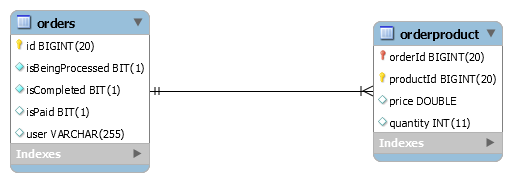
\includegraphics[height=3.5cm, width=15.7cm]{orderDB}
\end{figure}

Dodatkowe uwagi:
\begin{enumerate}
\item pole "orderId" jest generowane automatycznie
\item żadne pole OrderProduct nie może być null'em - w przeciwnym wypadku odpowiedź od serwisu produktów nie pozwoli na utworzenie takiego zapytania
\end{enumerate}




%\clearpage
\newpage
\subsection{Frontend}
Interfejs graficzny sklepu zostanie zrealizowany jako stron a internetowa pozwalająca na interakcję użytkowników z systemem. Pozwala klientom na logowanie, wylogowanie oraz rejestrację. Do realizacji zostaną wykorzystane biblioteki oraz framework Vue.js, Vuex, Bootstrap, Bootstrap Vue, npm i vue-sessionstorage.

\begin{figure}[] 
  %\label{ fig7} 
  \begin{minipage}[b]{0.5\linewidth}
  	\caption{Główne składowe sklepu.}
  	\label{mainpage}
    \centering
    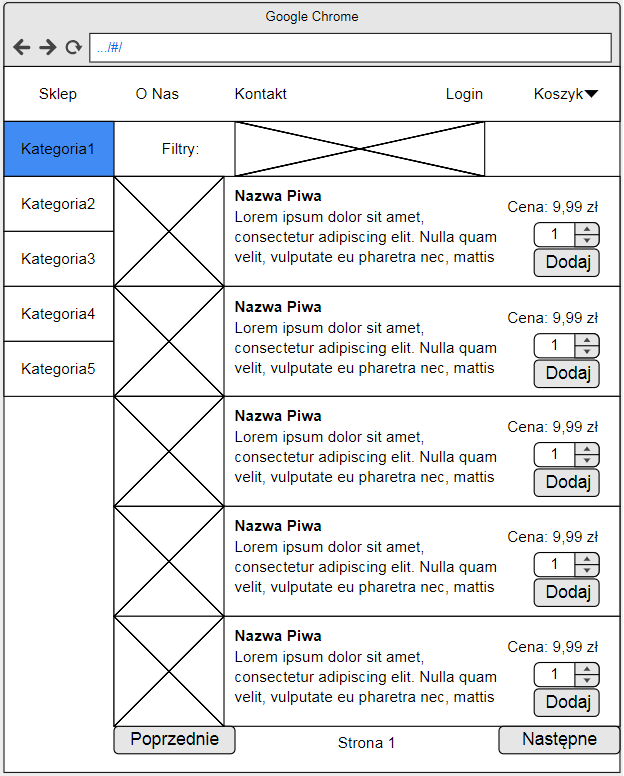
\includegraphics[height=8.15cm, width=.75\linewidth]{mainpage} 
    \vspace{4ex}
  \end{minipage}%%
  \begin{minipage}[b]{0.5\linewidth}
  	\caption{Tworzenie koszyka produktów.} 
  	\label{opencart}
    \centering
    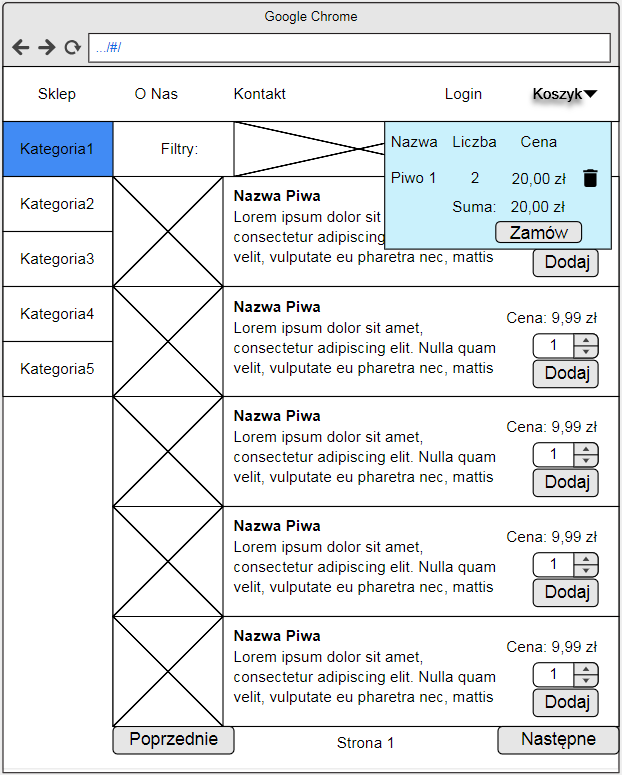
\includegraphics[height=8.15cm, width=.75\linewidth]{opencart} 
    \vspace{4ex}
  \end{minipage} 
  \begin{minipage}[b]{0.5\linewidth}
  	\caption{Zatwierdzanie koszyka produktów.} 
  	\label{finalizingcart}
    \centering
    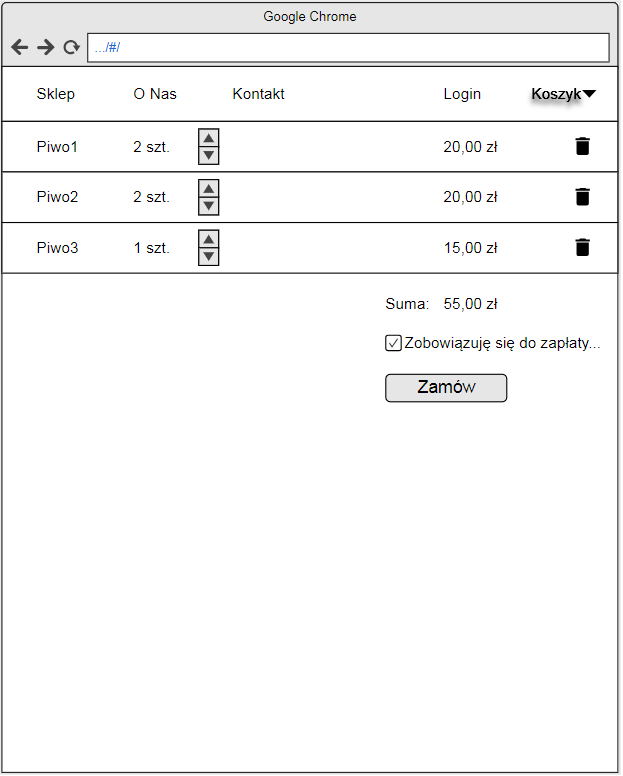
\includegraphics[height=8.15cm, width=.75\linewidth]{finalizingcart} 
    \vspace{4ex}
  \end{minipage}%% 
  \begin{minipage}[b]{0.5\linewidth}
  	\caption{Strona logowania/rejestracji.} 
  	\label{login}
    \centering
    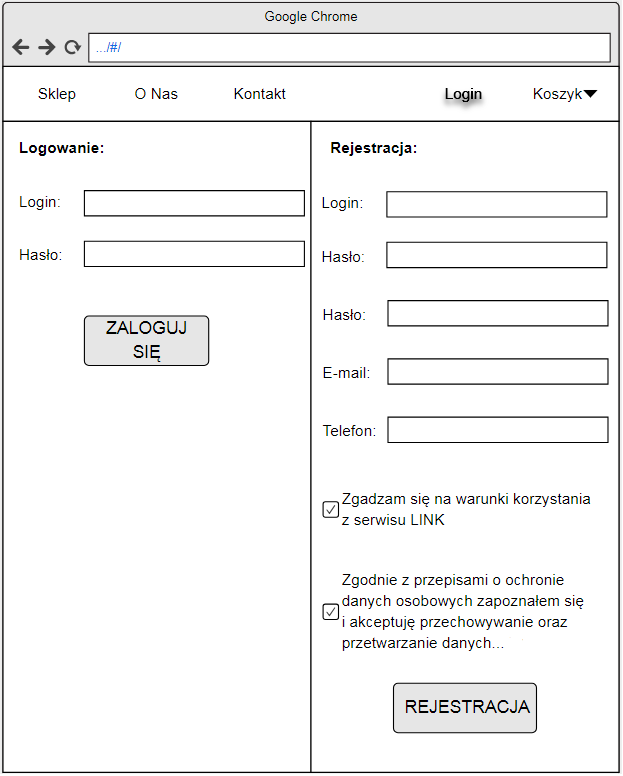
\includegraphics[height=8.15cm, width=.75\linewidth]{login} 
    \vspace{4ex}
  \end{minipage} 
\end{figure}

Menu nawigacyjne widoczne na diagramie zawiera 5 odnośników do głównych komponentów strony:
\begin{enumerate}
\item Sklep -- składa się z głównych części, widocznych na diagramie \ref{mainpage}:
\begin{itemize}
\item Pionowe menu kategorii: Naciśnięcie dowolnej kategorii spośród dostępnych w menu pobiera informacje o dostępnych produktach tej kategorii oraz wyświetla je w przestrzeni na karty produktów. Informacje o istniejących kategoriach pobierane są z serwisu produktów.
\item Przestrzeń kart produktów: Po  wybraniu kategorii produktów wyświetlane są tu karty zawierające informacje o poszczególnych produktach. Dane produktów pobierane są z serwisu produktów i zawierają takie informacje jak nazwa produktu i cena, a także pozwalają na dodanie produktu do koszyka.

Na raz wyświetlana jest tylko jedna strona produktów zawierająca ograniczoną ich liczbę. Do wyświetlenia innej strony produktów należy wybrać odpowiednią opcję na dole przestrzeni kart produktów.
\end{itemize}

\item Podstrona ,,O nas" -- zawiera informacje o zespole/sklepie.
\item Podstrona ..Kontakt" -- zawiera informacje kontaktowe
\item Koszyk -- Wybór tej opcji prowadzi do strony koszyka (diagram \ref{opencart}) pozwalającej na zmianę ilości produktów znajdujących się w koszyku, usuwania produktów z koszyka oraz zaakceptowania koszyka.

Stan koszyka przechowywany jest  w stanie aplikacji webowej. Użytkownik może dodawać oraz usuwać produkty z koszyka. Dodawanie przeprowadzane jest poprzez naciśnięcie przycisku dodawania do koszyka pożądanego produktu w sklepie. Z koszyka można usunąć produkt naciskając odpowiedni przycisk w wysuwanym menu koszyka.

W wysuwanym menu koszyka znajduje się również przycisk przenoszący użytkownika do ostatecznego wyboru zamówienia. Na tej stronie (diagram \ref{finalizingcart}) możliwe jest usuwanie przedmiotów z koszyka, jak również wysłanie zamówienia do serwisu. Żeby możliwe było wysłanie zamówienia do serwisu wymagane jest wcześniejsze zalogowanie.

Po zaakceptowaniu koszyka oraz otrzymaniu informacji zwrotnej z serwisu zamówień o utworzeniu zamówienia - koszyk jest czyszczony. W przypadku błędnych danych w zamówieniu takich jak niewystarczający stan w magazynie - użytkownik jest informowany.
\item Logowanie -- Jeśli użytkownik jest niezalogowany w menu nawigacyjnych znajduje się odnośnik do strony Logowania/Rejestracji. W przeciwnym razie znajduje się tam nazwa użytkownika oraz odnośnik do procedury wylogowania.

Na podstronie logowania (diagram \ref{login}) znajdują się 2 odseparowane od siebie formularze. Formularz logowania zawiera w sobie miejsce na wpisanie loginu i hasła oraz przycisk logowania.

Formularz Rejestracji składa się z pól pozwalających na rejestrację użytkownika oraz przycisku rejestracji.
\end{enumerate}

Strony internetowe wykorzystujące framework Vue.js zbudowane są z zagnieżdżonych w sobie komponentów. Budowę strony obrazuje diagram \ref{frontendUML} . Element "Router" na podstawie ścieżki w adresie URL wyświetla odpowiednio różne komponenty. Dzięki takiej budowie strony przejście między podstronami odbywa się bez przeładowania całej strony, mimo zmiany adresu URL.

\begin{figure}[ht]
%\vspace{-20pt}
\caption{Budowa strony sklepu.}
\label{frontendUML}
\centering
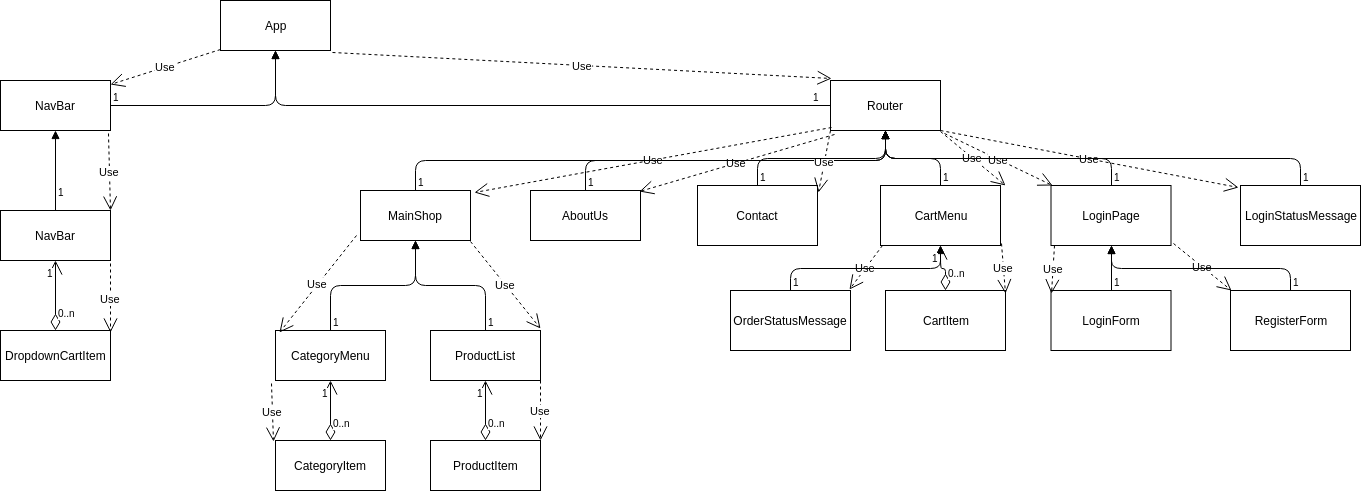
\includegraphics[height=6.5cm, width=15.7cm]{FRONTEND_UML}
\end{figure}

\newpage
%\subsection{Specyfikacja sprzętu i oprogramowania}
%\color{red}
%Na czym system powinien stać (sprzęt), systemy operacyjne, BD, przeglądarki internetowe
%\color{black}
\subsection{Specyfikacja technologii realizacji oprogramowania}

\subsubsection{Standaryzacja zapytań}
\label{stdZapytan}
Do wyszukiwania obiektów w każdym z serwisów wykorzystywany jest parser generujący z parametru w postaci napisu zapytanie do bazy danych.

Dostępne są trzy parametry:
\begin{enumerate}
\item filter -- definiuje po jakich polach i w jaki sposób filtrowane będą wyniki. Jego postać to:
\begin{lstlisting}
?filter=(kolumna1=(operator:wartosc1);kolumna2=(operator:wartosc2))
\end{lstlisting}
\vspace{-20pt}
Dostępne są operatory:
\begin{itemize}
\item eq/ne/lt/gt/le/ge -- równy / nierówny / mniejszy/ większy / mniejszy lub równy / większy lub równy
\item in -- wartość kolumny jest równa jednej z podanych wartości (podane w nawiasach, oddzielone przecinkiem), np. ?filter=(name=(in:(abc,bca,cba))
\item lk -- operator LIKE, można go stosować tylko do napisów
\end{itemize}

\item sortBy -- definicja po jakiej kolumnie i w jaki sposób (ASC / DESC - rosnąco / malejąco) sortowane będą wyniki
\begin{lstlisting}
?sortBy=(kolumna,kolejnosc)
\end{lstlisting}
\vspace{-20pt}

\item page -- definicja paginacji wyników. Podajemy w nim dwie wartości: numer od którego mają zaczynać się wyniki oraz liczbę zwróconych wyników.

\begin{lstlisting}
?page=(pierwszyWynik,liczbaWynikow)
\end{lstlisting}
\vspace{-20pt}

Wyniki numerowane są od zera. Przykładowo jeśli chcemy wyświetlić wyniki podzielone na dwie strony po 25 wyników, by uzyskać pierwszą należy podać: ?page(0,25). Otrzymamy wtedy wyniki o numerach 0 - 24. Aby uzyskać kolejną stronę (wyniki 25 - 49) należy podać: ?page=(25,25).
\end{enumerate}

Przykładowe zapytanie do serwisu produktów:
\begin{lstlisting}
?filter=(price=(le:15.45);price=(ge:5.00);quantity=(gt:0))&sortBy=(name,ASC)&page=(0,25)
\end{lstlisting}
\vspace{-20pt}
zwróci 25 pierwszych produktów, których w sklepie jest więcej niż 0 sztuk, ich cena jest większa od 5.00, a także mniejsza lub równa 15.45. Będą one posortowane rosnąco.

%W czym piszemy system? Słówko o dockerach, front/back-end, administracja systemem
\section{Właściwości niezawodności i bezpieczeństwa}
\subsection{Keycloak}
Keycloak jest oprogramowaniem open source, zajmującym się obsługą zarządzania danymi użytkowników oraz ich autoryzacji w serwisach. Dodatkowymi funkcjonalnościami udostępnianymi przez program jest możliwość skonfigurowania federacji użytkowników (np. synchronizacja z bazą użytkowników LDAP), a także ustalenia tożsamości na podstawie tokenów otrzymanych przez inne systemy autoryzacyjne (np. Kerberos). Autoryzacja w Keycloak'u bazuje na protokołach OpenID Connect, OAuth 2.0 lub SAML. 

\subsubsection{Autoryzacja przy pomocy tokenów OpenID}

Standardową formą autoryzacji jest stworzenie lokalnej bazy dla danych użytkowników, z których następnie korzystać będzie aplikacja. Problemem, który stwarza to rozwiązanie jest oczywiście konieczność stworzenia oddzielnego konta dla użytkownika w każdej z naszych aplikacji. Oznacza to nie tylko konieczność utrzymania wszystkich instancji baz danych, ale jest także nużące dla samego użytkownika. Dodatkowo, ponieważ dane użytkownika powielone są w wielu miejscach, trudno jest zapewnić, iż nie będą miały do nich dostępu osoby niepowołane, a usunięcie danych z każdej z baz także nie byłoby trywialnym zadaniem.

Intuicyjnym rozwiązaniem, adresującym te problemy, jest stworzenie centralnej bazy użytkowników, z której korzystać będą wszystkie nasze aplikacje. Jednakże udzielenie bezpośredniego dostępu do jednej bazy danych wielu aplikacjom, których implementacje korzystania z niej mogą się różnić, także nie wydaje się być zbyt atrakcyjne, szczególnie w przypadku tak wrażliwych danych. Zamiast tego wykorzystuje się wyspecjalizowane serwisy, odpowiadające za autoryzację oraz zarządzanie danymi użytkowników. Można zadać sobie pytanie, czy tego typu rozwiązanie nie powoduje stworzenia pojedynczego modułu, którego awaria spowoduje brak możliwości dostępu do wszystkich aplikacji. By temu zapobiec należy zapewnić jego redundancję, co można osiągnąć wykorzystując tokeny OIDC.

W ogólności rozwiązanie to wygląda następująco - do serwisu zarządzającego danymi użytkownika wysyłane jest żądanie, w którym zawierane są informacje pozwalające potwierdzić jego tożsamość (standardowo nazwa użytkownika oraz hasło). W odpowiedzi zwracany jest token, zakodowany zgodnie ze standardem RFC 7519 (JSON Web Token) i podpisany przez wystawiający go serwis, który zawiera w sobie m.in. dane o tożsamości jego posiadacza,  jednostce wydającej token oraz czasie jego ważności. Token może następnie posłużyć do stwierdzenia czy użytkownik posiada dostęp do żądanych przez niego zasobów. Ponieważ może on też być przekazywany dalej do innych aplikacji, nie ma konieczności oddzielnego logowania użytkownika w każdej z nich, o ile wszystkie są skonfigurowane tak, by móc połączyć się z serwisem zarządzającym autoryzacją i potwierdzić autentyczność tokena.

Przy wykorzystaniu tokenów nie mamy więc do czynienia ze standardową sesją, której dane są przechowywane na serwerze - użytkownik autoryzowany jest poprzez sprawdzenie tokena zapisanego w pamięci, który może być używany do czasu jego wygaśnięcia. Dopóki token nie zostanie przedawniony, możliwe jest jego odświeżenie, czego obsługą zajmuje się serwer aplikacji (zakładając, iż użytkownik cały czas z niej korzysta).

Serwisem zarządzającym danymi użytkowników oraz obsługującego wystawianie tokenów jest w naszym projekcie Keycloak. Jako oprogramowanie open source, może on zostać użyty do zapewnienia bezpieczeństwa bez konieczności zakupu bardziej kosztownych rozwiązań, a równocześnie z pewnością użycie go jest preferowane w stosunku do alternatywy, którą byłaby konieczność samodzielnej implementacji tego typu serwisu. Ponieważ należy on do grupy projektów firmy RedHat, daje to nadzieję, iż będzie on wciąż rozwijany i dostosowywany do aktualnych potrzeb na rynku. Dodatkową zaletą jest aktualizowany regularnie przez twórców obraz Docker, co zdecydowanie ułatwia instalację oraz utrzymanie.

\subsubsection{Keycloak w kontekście RODO}

Część z zalet, które skłaniają do wykorzystania serwisu Keycloak w kontekście RODO została już podana w poprzedniej części. Przede wszystkim ustalenie centralnej bazy użytkowników i jednego punktu dostępu pozwala na dokładną kontrolę tego czy są one odpowiednio przechowywane oraz czy dostęp do nich mają jedynie odpowiednie jednostki. Przy pobieraniu czy sprawdzaniu tokena nie są w żaden sposób przesyłane prywatne dane użytkowników - są one udostępniane jedynie na żądanie. Hasła użytkowników są haszowane, a inne serwisy w razie potrzeby powiązania użytkowników np. z zamówieniami używają w tym celu GUID, który jest zgodny ze standardem RFC 4122. Ponieważ identyfikator ten w tabelach poszczególnych serwisów nie jest kluczem obcym, możliwe jest usunięcie użytkownika bez naruszania ich działania (konieczne jest jedynie obsłużenie wyświetlenia komunikatu o braku danego użytkownika w bazie danych), udostępniona jest także możliwość edycji jego danych personalnych. Keycloak może też zostać łatwo skonfigurowany tak by wykorzystywać przy transferze danych certyfikaty SSL.

\subsubsection{Użytkowanie w projekcie}

W ramach konfiguracji należy zdefiniować dla każdego z serwisów klienta, dla którego wygenerowany zostanie secret w postaci guida (przykładowo e7b70cf3-8d73-466b-8592-b8cfea69f704). Każdy z serwisów łączyć się będzie ze swoim klientem, podając odpowiedni secret.

Autoryzacja użytkowników w serwisach przebiegać będzie następująco:
\begin{enumerate}
\item Przy logowaniu użytkownika, do serwera Keycloak wysyłane jest zapytanie wraz z podanymi loginem oraz hasłem użytkownika. W odpowiedzi zwracany jest token JWT, w którym zawierana jest m.in. informacja o id użytkownika, posiadanych przez niego rolach, oraz czasie wygaśnięcia tokena. Dodatkowo podawany jest refresh token, który pozwoli pobrać nowy token dostępu dla tego samego użytkownika, o ile zostanie podany przed czasem wygaśnięcia (w innym przypadku konieczne jest ponowne zalogowanie przez użytkownika).
\item Otrzymany token jest podawany w zapytaniach do serwisów (w nagłówku Authorization). W serwisach sprawdzane jest, czy token nie wygasł, został wystawiony przez odpowiedniego wystawcę oraz (na podstawie ról) czy użytkownik ma dostęp do danego zasobu. W razie potrzeby możliwe jest dodanie ręcznie zdefiniowanych pól w tokenie, które następnie mogą być sprawdzone w samym serwisie.
\item W przypadku gdy konieczna jest komunikacja między serwisami, przekazują one dalej w zapytaniach otrzymany token.
\end{enumerate}

Przykład pobierania tokena przedstawia rysunek \ref{pobieranieTokena}. Na diagramie \ref{zapytanieZTokenem} widać wysyłanie zapytania z tokenem w nagłówku.

\begin{figure}[ht]
%\vspace{-20pt}
\caption{Zapytanie pobierające token.}
\label{pobieranieTokena}
\centering
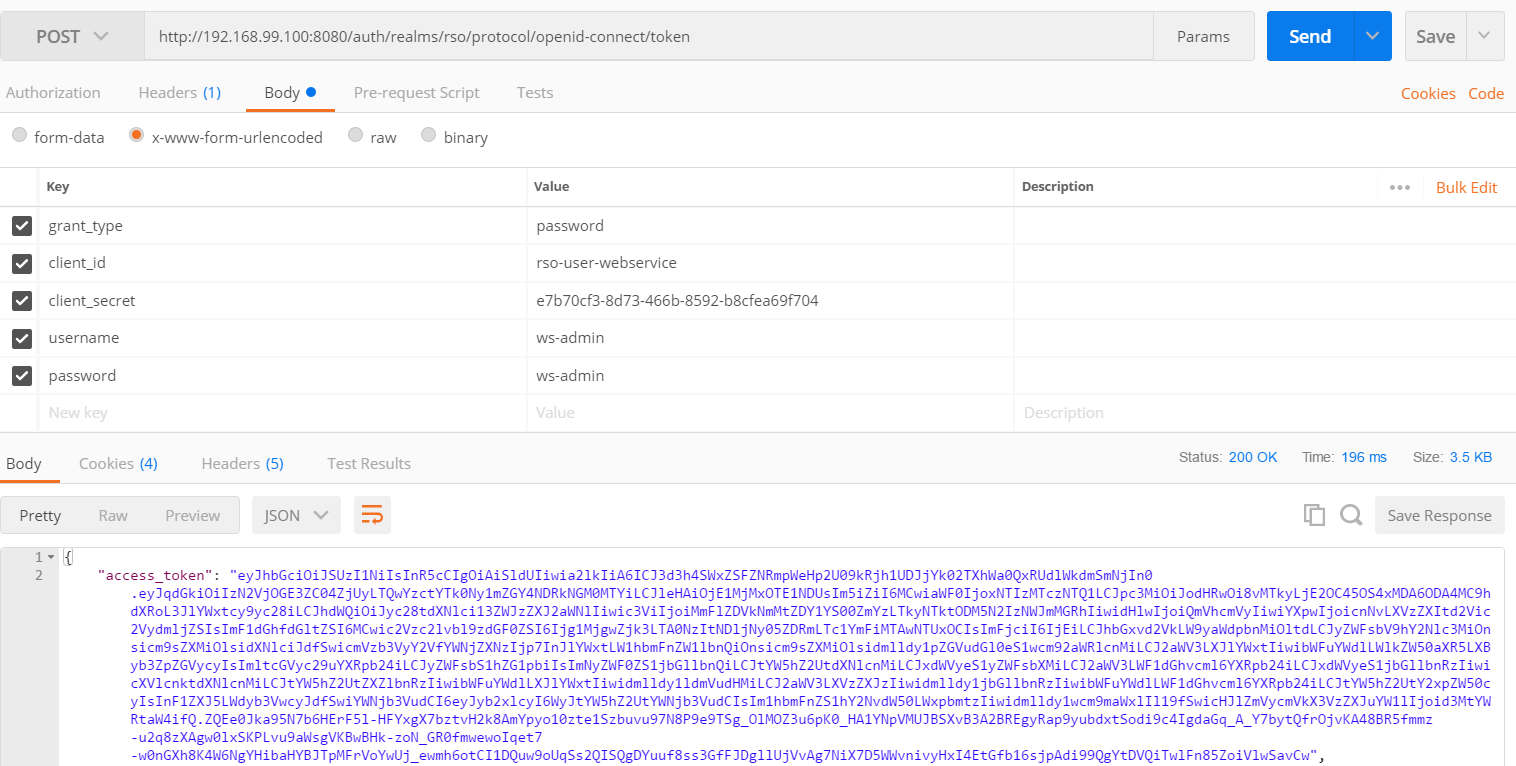
\includegraphics[height=8.cm, width=15.7cm]{requestForToken}
\end{figure}

\begin{figure}[ht]
%\vspace{-20pt}
\caption{Zapytanie zawierające token w nagłówku.}
\label{zapytanieZTokenem}
\centering
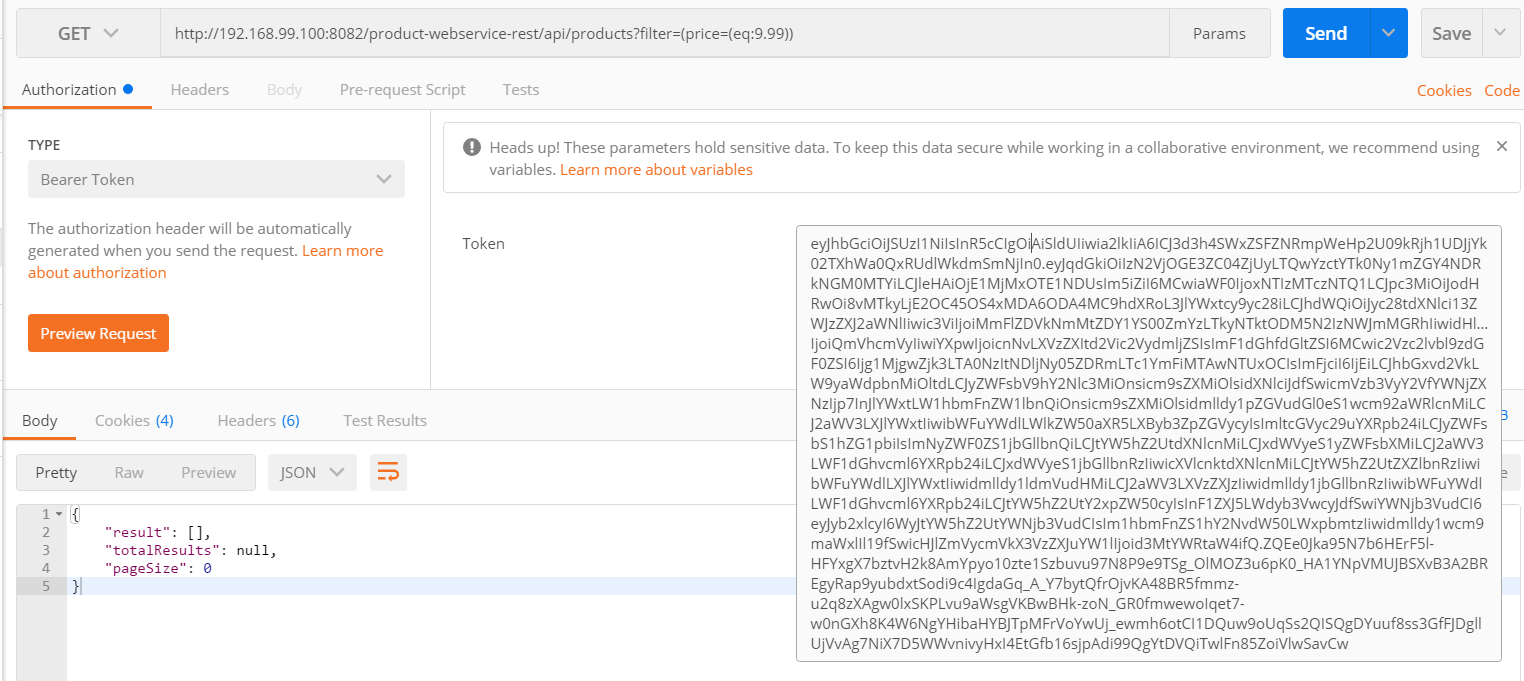
\includegraphics[height=9cm, width=15.7cm]{requestWithToken}
\end{figure}

Poniżej przedstawiony jest plik konfiguracyjny w serwisie (keycloak.json):

\begin{lstlisting}
{
  "realm": "rso",
  "auth-server-url": "http://192.168.99.100:8080/auth",
  "ssl-required": "external",
  "resource": "rso-user-webservice",
  "credentials": {
    "secret": "e7b70cf3-8d73-466b-8592-b8cfea69f704"
  }
}
\end{lstlisting}
\vspace{-20pt}
Konfiguracja pliku web.xml tak, aby konieczne było posiadanie roli user w celu uzyskania dostępu do dowolnego REST-a:

\begin{lstlisting}
<web-app version="2.4" xmlns="http://java.sun.com/xml/ns/j2ee"
         xmlns:xsi="http://www.w3.org/2001/XMLSchema-instance"
         xsi:schemaLocation="http://java.sun.com/xml/ns/j2ee http://java.sun.com/xml/ns/j2ee/web-app_2_4.xsd">

    <login-config>
        <auth-method>KEYCLOAK</auth-method>
    </login-config>

    <security-role>
        <role-name>user</role-name>
    </security-role>

    <security-constraint>
        <web-resource-collection>
            <web-resource-name>user-webservice</web-resource-name>
            <url-pattern>/*</url-pattern>
        </web-resource-collection>
        <auth-constraint>
            <role-name>user</role-name>
        </auth-constraint>
    </security-constraint>
</web-app>
\end{lstlisting}
\vspace{-20pt}
\subsection{Replikacja baz danych}
Serwisy stworzone w projekcie wykorzystują bazy danych MySQL. Replikacja w MySQL pozwala na odwzorowanie danych z nadrzędnego serwera bazodanowego (ang. master) na jeden lub wiele podrzędnych serwerów (ang. slave). Replikacja domyślnie odbywa się asynchronicznie, dzięki czemu serwery podrzędne nie muszą być podłączone permanentnie, aby otrzymywać aktualizacje. To sprawia, że replikacja może odbywać się na dalekich dystansach, bądź też przez tymczasowe lub ulotne połączenie. W zależności od konfiguracji, replikacja może dotyczyć wszystkich baz danych, wybranych, a nawet konkretnych tabel wewnątrz bazy. Replikacja w MySQL jest najbardziej korzystna dla systemów procesujących częste odczyty i rzadkie zapisy.

\begin{figure}[ht]
%\vspace{-20pt}
\caption{Replikacja baz danych.}
\label{replikacja}
\centering
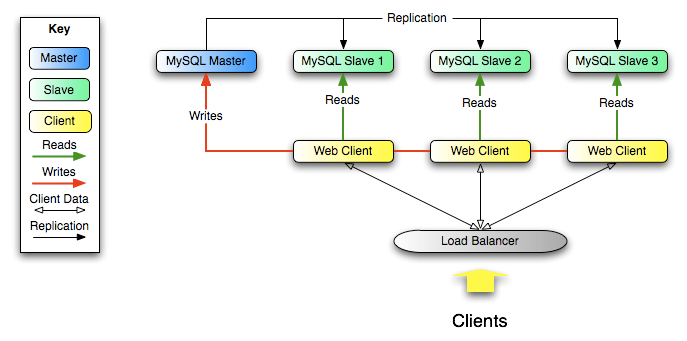
\includegraphics[height=9cm, width=15.7cm]{replikacja}
\end{figure}

Do zalet replikacji MySQL można zaliczyć:
\begin{itemize}
\item Skalowalność: w omawianym środowisku, wszyskie operacje zapisu nadal muszą odbywać się na serwerze nadrzędnym, jednak już operacje odczytu - niekoniecznie. Ten model poprawia wydajność obu operacji, jako że wówczas serwer nadrzędny może być oddany jedynie operacjom zapisu, podczas gdy operacje odczytu są rozłożone na serwery podrzędne.
\item Bezpieczeństwo danych: jako, że dane są powtórzone na serwerach podrzędnych, nie tylko przetrwają one awarię pojedyńczego węzła, ale również jest możliwym wykonywanie kopii zapasowych bez znaczącego wpływu na działanie serwisu.
\item Analityka: analiza informacji składowanych w bazie danych może odbywać się na jednym z serwerów podrzędnych, wskutek czego serwer nadrzędny pozostaje nieobciążony dodatkową pracą.
\item Stabilność serwisu: w przypadku awarii serwera nadrzędnego, jeden z serwerów podrzędnych może przejąć jego obowiązki.
\end{itemize}

\subsubsection{Implementacja}
Zasada działania replikacji jest oparta o serwer nadrzędny śledzący wszystkie zmiany w bazie danych w dzienniku (ang. log). Dziennik ten zawiera informacje o wszystkich operacjach, które modyfikują strukturę bazy danych lub same dane od momentu, w którym serwer został uruchomiony.

Każdy serwer podrzędny, który łączy się z serwerem nadrzędnym, pobiera z niego kopię wspomnianego dziennika. Na jego podstawie odgrywa wszystkie wydarzenia jakie miały miejsce na  serwerze nadrzędnym, w ten sposób synchronizując się z serwerem nadrzędnym.

Każdy z serwerów podrzędnych jest niezależny od siebie, wskutek czego odczyt logu z serwera nadrzędnego również odbywa się niezależnie. Dzięki temu, każdy z serwerów podrzędnych dokonuje synchronizacji w swoim własnym tempie i częstotliwości, zależnym od parametrów sprzętu i jakości połączenia.

\subsubsection{Więzy spójności}
Replikacja w systemie MySQL jest domyślnie asynchroniczna, toteż odczyty z węzłów podrzędnych siłą rzeczy muszą być opóźnione. Po zakończeniu transakcji przez serwer nadrzędny musi ona być bowiem zapisana w dzienniku, który później zostanie pobrany przez serwer podrzędny w celu odtworzenia wydarzenia. MySQL zapewnia atomowość operacji - użytkownik może odczytać stare dane, jednak istnieje gwarancja, że będą one spójne. Wymaga to zachowania ostrożności w systemach wymagających odczytu aktualnych danych.

\subsubsection{ProxySQL}
ProxySQL służy jako pośrednik pomiędzy serwerem MySQL a aplikacjami które sięgają do jego baz danych, jak również rozdziela ruch pomiędzy dostępnymi serwerami. W ten sposób dostarcza aplikacjom jednolity interfejs dostępu do serwerów podrzędnych w celach odczytu danych, nawet w sytuacjach ich częściowej awarii.

\subsection{Zarządzanie instancjami serwisów}
Wykorzystanie aplikacji Docker pozwala na upewnienie się w łatwy sposób, iż we wszystkich instancjach naszego programu działa jego odpowiednia wersja, a ich restart nie będzie sprawiał trudności. Jednakże w przypadku potrzeby automatyzacji skalowania aplikacji, konieczne jest stworzenie serwisu pełniącego rolę zarządcy. Główne zadania które do niego należą są następujące:

\begin{itemize}
\item Utrzymanie przez cały czas określonej liczby instancji poszczególnych serwisów. Zawiera się w tym zarówno tworzenie/usuwanie instancji na żądanie, jak i zatrzymywanie oraz uruchamianie nowych w przypadku awarii. W przypadku zmiany wersji obrazu danego serwisu najpierw uruchamiane są dodatkowe instancje zawierające aplikacje w nowej wersji, a następnie wyłączane są poprzednie, tak by zapewnić płynne przejście do nowej wersji. Dodatkowo konieczne jest rozmieszczenie instancji serwisów na udostępnionych dla zarządcy maszynach, tak by odpowiednio rozdysponować dostępne zasoby sprzętowe.
\item Udostępnienie pod stałym adresem dostępu do danego serwisu oraz odpowiednie zarządzanie zapytaniami, tak by do poszczególnych instancji trafiała optymalna ich liczba.
\item Przechowywanie zmiennych środowiskowych, które następnie rozprowadzane są do instancji odpowiednich serwisów. Są to m.in. adresy pozostałych serwisów oraz adresy i hasła do odpowiednich baz danych.
\end{itemize}

Kubernetes spełnia wszystkie z powyższych wymagań - jest to system udostępniony na zasadach open source, przystosowany do wystawiania oraz skalowania aplikacji zawartych w obrazach Docker. Po skonfigurowaniu w prosty sposób można określić, jakie obrazy mają zostać uruchomione, pod jakimi adresami mają zostać udostępnione oraz jaka ma być liczba ich instancji. Poszczególne serwisy komunikują się między sobą w zabezpieczonej sieci wewnętrznej, możliwe jest także skonfigurowanie połączenia między klientem a proxy serwisów z użyciem SSL. Zmienne środowiskowe mogą zostać zapisane w mapie konfiguracji, tak by przykładowo zmiana adresu bazy danych w tejże mapie spowodowała jego zmianę we wszystkich serwisach. Możliwe jest także odczytywanie logów oraz uzyskanie dostępu do konsoli poszczególnych instancji, jednak do zbierania logów ze wszystkich instancji danego serwisu konieczne jest użycie dedykowanych aplikacji (np. Logstash i Kibana).

\section{Organizacja projektu}
\subsection{Możliwe rozszerzenia}
W ramach projektu, sklep internetowy będzie realizował transakcje między klientami a sklepem. Funkcjonalność ta realizowana jest przez trzy serwisy opisane wyżej.

Rozwój projektu może obejmować:
\begin{enumerate}
\item Obsługę zamówienia po stronie dostawców:
\begin{itemize}
\item zmiana stanów zamówienia w zależności od tego czy zamówienie jest realizowane/transportowane/zakończone
\item realizacja umów zawartych z dostawcami -- nowy serwis dostaw, którego zadaniem jest realizacja zamówienia złożonego przez klienta (który dostawca realizuje które zamówienie)
\end{itemize}
\item Realizację płatności -- zamiast korzystania z zewnętrznego serwisu
\item Obsługę reklamacji i zwrotów -- nowy mikroserwis
\item Generowanie raportów i statystyk zgodnie z WF6.
\end{enumerate}

Obecnie istniejące serwisy przygotowane są w taki sposób by obsługa zamówień po stronie dostawców nie wymagała ich modyfikacji (lub bardzo mało).

%\color{red}
%\section{Instrukcja użytkownika systemu}
%przyda się przy dokumentacji końcowej

%Etapy projektu\\
\subsection{Etapy projektu}
\begin{table}[ht]
\label{etapyProjektu}
\centering
\begin{tabularx}{\textwidth}{|l|X|}
\hline
 \multicolumn{1}{|c|}{Data} & \multicolumn{1}{c|}{Treści spotkania} \\\hline
 13.03.2018 & Utworzenie zespołu, wybór i zgłoszenie tematu projektu \\\hline
 22.03.2018 & Ustalenie organizacji zespołu, ustalenie wstępnych założeń projektowych, zarys koncepcji rozwiązania \\\hline
 29.03.2018 & Specyfikacja i analiza wymagań systemowych, opracowanie architektury rozwiązania \\\hline
 04.04.2018 & Przydział zadań pomiędzy członków zespołu \\\hline
 05.04.2018 & Utworzenie repozytorium kodu na potrzebę projektu, rozpoczęcie wstępnych implementacji serwisów \\\hline
 19.04.2018 & Pierwsze próby doprecyzowanie interfejsów serwisów i wyglądu aplikacji użytkowej \\\hline
 26.04.2018 & Szczegółowy opis wykorzystywanych narzędzi i technologii \\\hline
 06.05.2018 & Redakcja i edycja dokumentacji \\\hline
\end{tabularx}
\end{table}

%Przydział zadań\\
%Co udało się zrealizować, a czego nie\\
%Podsumowanie prac i wnioski\\






%\clearpage
%\newpage
%\begin{thebibliography}{9}
%%\addcontentsline{toc}{section}{Literatura}
%%\bibitem{BOCD}
%%Z. Michalewicz, D. B. Fogel
%%\emph{Jak to rozwiązać czyli nowoczesna heurystyka}.
%%WNT, Warszawa 2006
%\bibitem{knapsack}
%\url{http://www-users.mat.uni.torun.pl/~henkej/knapsack.pdf}
%\bibitem{knapsack2}
%\url{http://pe.org.pl/articles/2014/6/37.pdf}
%\bibitem{knapsack3}
%\url{http://home.agh.edu.pl/~slukasik/pub/021_Lukasik_KAEiOG2011(presentation).pdf}
%\bibitem{knapsack4}
%\url{https://eti.pg.edu.pl/documents/176546/25263566/SZ_wyklad2.pdf}

%\end{thebibliography}

\end{document}
